\documentclass[12pt,a4paper]{article}
\usepackage[utf8]{inputenc}
\usepackage[T1]{fontenc}
\usepackage{amsmath, amssymb}
\usepackage{geometry}
\usepackage{hyperref}
\usepackage{booktabs}
\usepackage{graphicx}
\usepackage{setspace}
\usepackage{caption}
\usepackage{float}
\graphicspath{{assets/}}
\geometry{margin=1in}
\setstretch{1.25}

\begin{document}

% Title Page
\begin{titlepage}
    \centering
    \Huge
    \textbf{Jaypee Institute of Information Technology, Sector - 62, Noida} \\
    \vspace{0.5cm}
    \Large
    \textbf{B.Tech CSE II Semester} \\
    \vspace{1cm}
    \vspace*{\fill}
    
\includegraphics[scale=2]{jiit_logo} \\
    \vspace{1.5cm}
    \Huge
    \textbf{Mathematics 2 PBL Report} \\
    \Large
    \textbf{Title : Fourier Series} \\
    \vspace{1cm}
    \Large
    \textbf{Submitted to} \\
    \textbf{Dr. Ram Surat Chauhan}\\
    \vspace{1cm}
    \textbf{Submitted by} \\
    \vspace{0.5cm}
    \begin{tabular}{ll}
        Mehul Gupta & 2401030224 \\
        Ananaya Shrivastav & 2401030230 \\
        Sara Jain & 2401030235 \\
        Aastha Malik & 2401030251 \\
        Mukul Aggarwal & 2401030239 \\
    \end{tabular}
    \vspace*{\fill}
    \normalsize
\end{titlepage}


% Letter of Transmittal
\begin{center}
    \Large\textbf{Letter of Transmittal}
\end{center}
\vspace{1cm}

\noindent
Dr. Ram Surat Chauhan \\
Department of Mathematics \\
Jaypee Institute of Information Technology \\
Sector - 62, Noida \\

\vspace{1cm}

\noindent
\textbf{Subject:} Submission of Report on \textquotedblleft Fourier Series\textquotedblright \\

\vspace{1cm}

\noindent
Dear Sir, \\

\vspace{1em}

\noindent
We are pleased to submit our report titled \textit{Fourier Series: Theory, Applications and Visualizations}, as part of the B.Tech CSE II Semester coursework. This report explores the theoretical foundation of Fourier series, its derivation, properties, and a variety of real-world applications including signal processing and heat transfer. It also includes graphical visualizations to support the concepts. \\

\vspace{1em}

\noindent
We hope this report meets your expectations and provides valuable insights into the mathematical and practical aspects of Fourier analysis. \\

\vspace{2em}
\noindent
Sincerely, \\
\vspace{1em}
\noindent
\begin{tabular}{rl}
    Mehul Gupta & 2401030224 \\
    Ananya Srivastava & 2401030230 \\
    Sara Jain & 2401030235 \\
    Mukul Aggarwal & 2401030239 \\
    Aastha Malik & 2401030251 \\
\end{tabular}

\newpage
\tableofcontents
\newpage

% Sections
\section{History}
The Fourier series is a mathematical tool used to express periodic functions as the sum of sine and cosine terms. The concept originated with Jean-Baptiste Joseph Fourier in the early 19th century. In 1807, Fourier introduced the idea while studying heat conduction problems in his work Théorie analytique de la chaleur. He proposed that any periodic function could be represented as an infinite sum of sines and cosines, breaking down complex waveforms into simpler components. This was revolutionary, as it allowed the analysis of heat and wave phenomena in a much more manageable form.
Fourier’s work faced initial criticism, but it gained acceptance and became foundational in fields such as signal processing, acoustics, and electrical engineering. The Fourier series has since become indispensable in mathematics, helping to solve partial differential equations and analyze periodic signals in various disciplines, including physics, engineering, and data science.


\section{Mathematical Foundation}
\subsection{Periodic Functions}
A function \( f(x) \) is periodic if \( f(x + T) = f(x) \) for all \( x \), where \( T \) is the period.

\subsection{Fourier Series Representation}
The Fourier series of a periodic function \( f(x) \) defined over \( [-L, L] \) is given by:
\[
f(x) = \frac{a_0}{2} + \sum_{n=1}^{\infty} \left( a_n \cos \frac{n\pi x}{L} + b_n \sin \frac{n\pi x}{L} \right)
\]
where the coefficients are:
\[
a_n = \frac{1}{L} \int_{-L}^{L} f(x) \cos\left( \frac{n\pi x}{L} \right) dx,\quad 
\quad b_n = \frac{1}{L} \int_{-L}^{L} f(x) \sin\left( \frac{n\pi x}{L} \right) dx
\]

\section{Types of Fourier Series}
\begin{itemize}
    \item \textbf{Full Range Fourier Series:} Defined on symmetric intervals.
    \item \textbf{Half-Range Sine Series:} Uses only sine terms, defined for odd extensions.
    \item \textbf{Half-Range Cosine Series:} Uses only cosine terms, defined for even extensions.
\end{itemize}

\section{Convergence of Fourier Series}
A Fourier series converges to \( f(x) \) at all points where \( f \) is continuous, and to \( \frac{f(x^-) + f(x^+)}{2} \) at points of discontinuity, as per Dirichlet conditions.

\section{Applications of Fourier Series}
\subsection{Signal Processing}
Fourier series are used to analyze and manipulate signals, such as in audio processing, image compression, and telecommunications. They help in filtering, compression, and noise reduction.

\subsection{Heat Equation}
Fourier series are used in solving heat conduction problems and fluid flow dynamics, particularly in cases involving periodic boundary conditions

\subsection{Electrical Engineering}
: In electrical circuits, Fourier series are used to analyze alternating current (AC) signals and waveforms. They help in understanding and designing filters, amplifiers, and oscillators

\subsection{Image Compression}
In image analysis, Fourier series are used for techniques like image compression, enhancement, and filtering. The Fourier transform can be applied to convert images into the frequency domain, allowing easier manipulation of noise and patterns.

\begin{figure}[H]
    \centering
    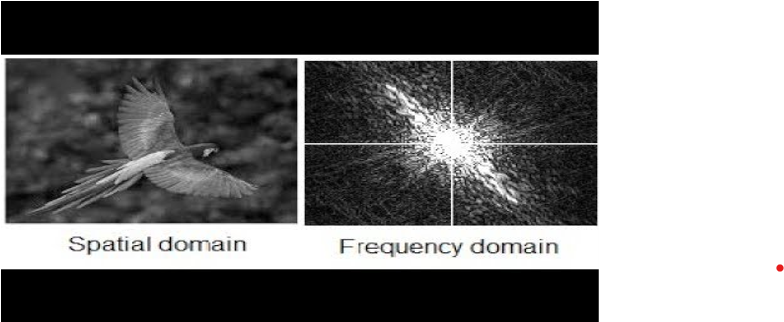
\includegraphics[width=0.7\textwidth]{image}
    \caption{image compression}
\end{figure}

\subsection{Control Systems}
: In control theory, Fourier series help model periodic inputs or disturbances in systems. It’s used to analyze the frequency response of systems and design controllers (like PID controllers) to ensure stability and performance

\subsection{Electromagnetic Theory}
In the study of electromagnetic waves, Fourier series are used to express waveforms, particularly in the context of periodic signals and their propagation through various mediums, like waveguides and antennas

\subsection{Fourier Analysis in Data Science}
Fourier series are used in time-series analysis to detect trends, cycles, and anomalies. In machine learning, Fourier transforms assist in feature extraction for pattern recognition, especially when dealing with periodic or cyclical data.

\subsection{ Mechanical Engineering}
In mechanical systems, Fourier series are applied to study forces and displacements in periodic systems like gears, engines, and rotating machinery. This helps engineers understand stress and strain distributions over time.

\subsection{Seismology}
: Fourier series are used in the analysis of seismic data to detect the frequency components of earth vibrations. This is crucial for understanding earthquakes and their impact on structures.
\begin{figure}[H]
    \centering
    \includegraphics[width=0.7\textwidth]{Seismology}
    \caption{Seismology}
\end{figure}

\subsection{Medical Imaging (MRI)}
In medical imaging technologies like MRI and CT scans, Fourier transforms (which extend the idea of Fourier series) are used to reconstruct images from raw data, converting information from the frequency domain back to the spatial domain.


\subsection{Astronomy}
Fourier series are used in the analysis of periodic signals from stars, planets, and other celestial objects. They help in understanding phenomena like stellar oscillations and cosmic microwave background radiation.

\begin{figure}[H]
    \centering
    \includegraphics[width=0.7\textwidth]{Astronomy}
    \caption{Astronomy}
\end{figure}



\section{Graphical Visualization}
\begin{figure}[H]
    \centering
    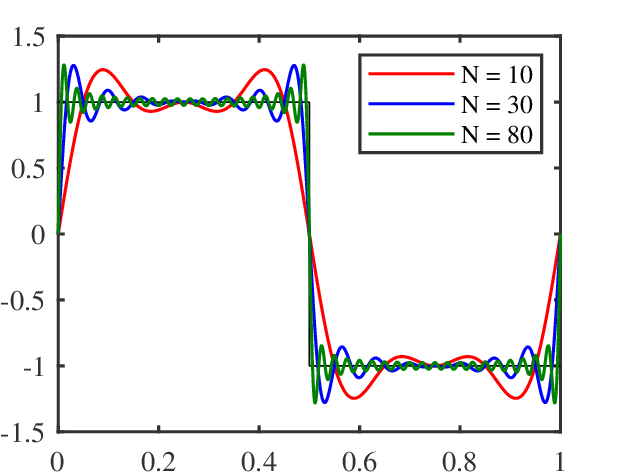
\includegraphics[width=0.7\textwidth]{fourier_square_wave}
    \caption{Approximation of square wave using Fourier series}
\end{figure}

The figure above illustrates how a Fourier series approximates a square wave using a finite number of terms. As the number of terms increases, the approximation becomes more accurate.

\section{Advantages and Limitations}
\subsection*{Advantages}
\begin{itemize}
    \item Decomposes complex signals into simpler components.
    \item Essential for digital signal processing.
\end{itemize}

\subsection*{Limitations}
\begin{itemize}
    \item Applicable only to periodic functions.
    \item Gibbs phenomenon near discontinuities.
\end{itemize}

\section{Conclusion}
In conclusion, Fourier series are an essential mathematical tool that has transformed various fields of science, engineering, and technology. Originating from Joseph Fourier's groundbreaking work on heat conduction, Fourier series enable the decomposition of complex periodic functions into simpler sinusoidal components, making analysis and manipulation much more manageable. The versatility of Fourier series is evident in their wide range of applications, from signal processing and electrical engineering to quantum mechanics, image processing, and even medical imaging. By breaking down waveforms and signals into constituent frequencies, Fourier series facilitate the study of vibrations, sound, heat, and much more. As the foundational principle for Fourier transforms, they continue to be indispensable in modern technology, contributing to advancements in data science, communication systems, and beyond. Fourier series remain a cornerstone in mathematics, providing powerful methods to solve real-world problems and drive innovation across multiple disciplines.

\section{References}
\begin{enumerate}
    \item Kreyszig, E. \textit{Advanced Engineering Mathematics}. Wiley.
    \item Boyce, DiPrima. \textit{Elementary Differential Equations}.
    \item \url{https://en.wikipedia.org/wiki/Fourier_series}
    \item \url{https://mathworld.wolfram.com/FourierSeries.html}
\end{enumerate}

\end{document}